\documentclass[a4paper,11pt]{article}
\usepackage[a4paper,total={18cm, 24cm}]{geometry}
\usepackage[parfill]{parskip}
\usepackage[utf8]{inputenc}
\usepackage[T1]{fontenc}
\usepackage{fancyhdr}
\usepackage[ddmmyyyy]{datetime}
\usepackage{graphicx}
\usepackage{subcaption}
\usepackage{multirow}
\usepackage{hyperref}
\usepackage{amsfonts}

\pagestyle{fancy}
\fancyhf{}
\lhead{\today}
\chead{Deep Learning - Initialization and Regularization}
\rhead{Jakub Rada}

\begin{document}
This homework assignment explores different means of initializing weights in a neural network and shows effects of bad initialization.
Also, it explores regularization by using dropout layers.

\section{Initialization - Deep Network}
First, we focus on initializing a deep network and see how the mean and variance of activations change during the forward pass and how the gradients propagate back.

We used the setup suggested on the website.
It is a network consisting of $50$ layers each with $512$ neurons.
The network has a parameter to determine which activation function is used, we experimented with \textit{ReLU} and \textit{tanh} activations.

The experiments were conducted in a way that for every specified pairs $(\mathrm{activation}, \mathrm{init method})$ we sampled a batch of $512$ vectors of size $512$, so that they can be passed directly to the input layer which has $512$ neurons.
Every vector was sampled from a normal distribution with mean $0$ and variance $1$.
After each layer (linear layer and activation after it), we computed and saved the mean and variance of the activation values over the whole batch.
Similarly for the backwards pass, we computed and displaed the mean and variance of each layer's gradients.
To implement the initializations we used the PyTorch built-in methods.

Next, we show the results for the selected combinations of initialization methods and activation functions and compare them.

\subsection{Original heuristic and \textit{tanh} activation}
This method is the oldest of the ones we tried.
The weights are initialized from a uniform distribution $U\left[-\frac{1}{\sqrt{n}}, -\frac{1}{\sqrt{n}}\right]$, where $n$ is the number of neurons in the previous layer.
In our case, where all the layers have the same size, the distribution is the same for all layers.

\begin{figure}[ht]
    \centering
    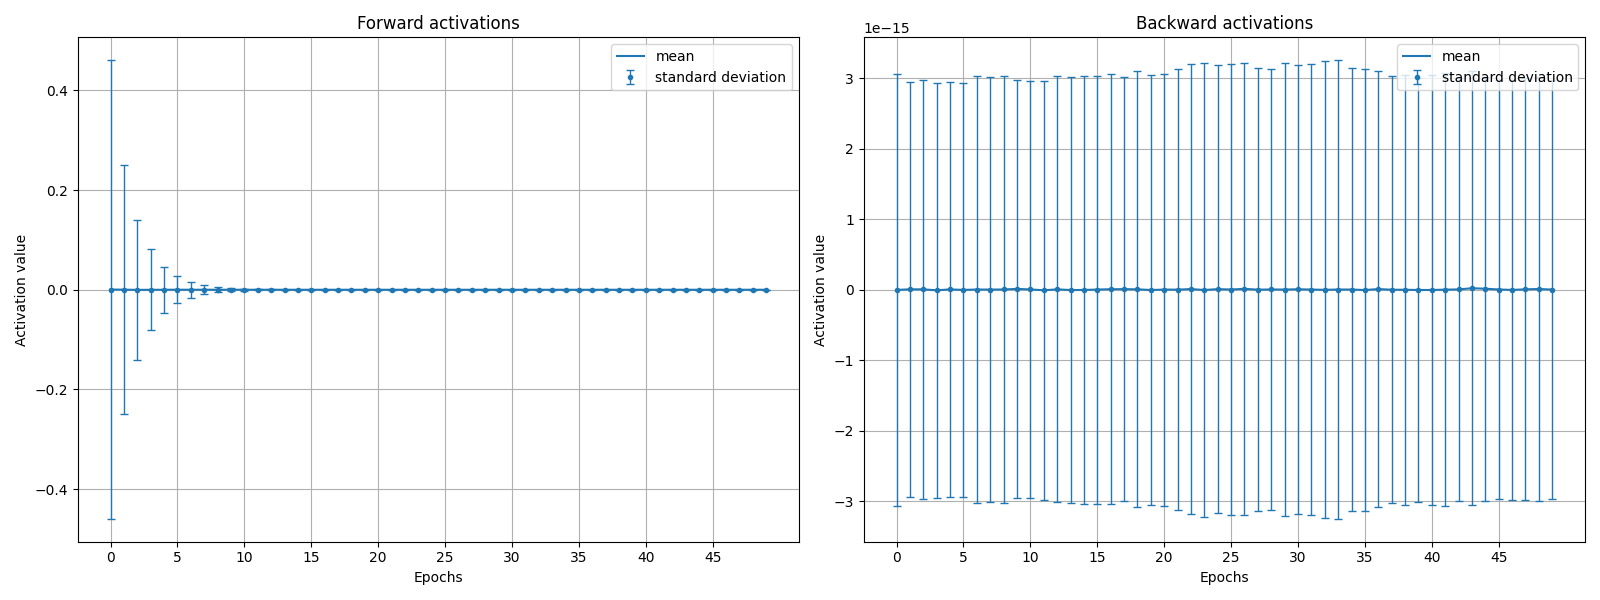
\includegraphics[width=0.95\textwidth]{../out/01_deep/tanh_original.png}
    \caption{Original heuristic initialization used with \textit{tanh} activation}
    \label{fig:orig_tanh}
\end{figure}

Figure \ref{fig:orig_tanh} shows the results of this combination.
We can immediately see that after a small number of layers the variance of the activations is very close to zero which is undesirable.
We would like the variance to be similar to the variance of the input data.
The gradients look better on the first glance becuase they have similar variances and zero mean, however they are very small.
In the graph we can see that the variance is of the order $10^{-15}$ which is almost zero.
Combined with some learning rate smaller than $1$, the learning would be extremely slow if any because the weights would be updated by such a small values.

\subsection{Xavier initialization}
A smart way to initialize the weights when using \textit{tanh} activation function is the \textbf{Xavier} method.
There are two versions of this method, one uniform and one normal, depending on the distribution from which the weights are sampled.
We compare both of them to see if there is any difference.

\begin{figure}[ht]
    \centering
    \begin{subfigure}[b]{0.95\textwidth}
        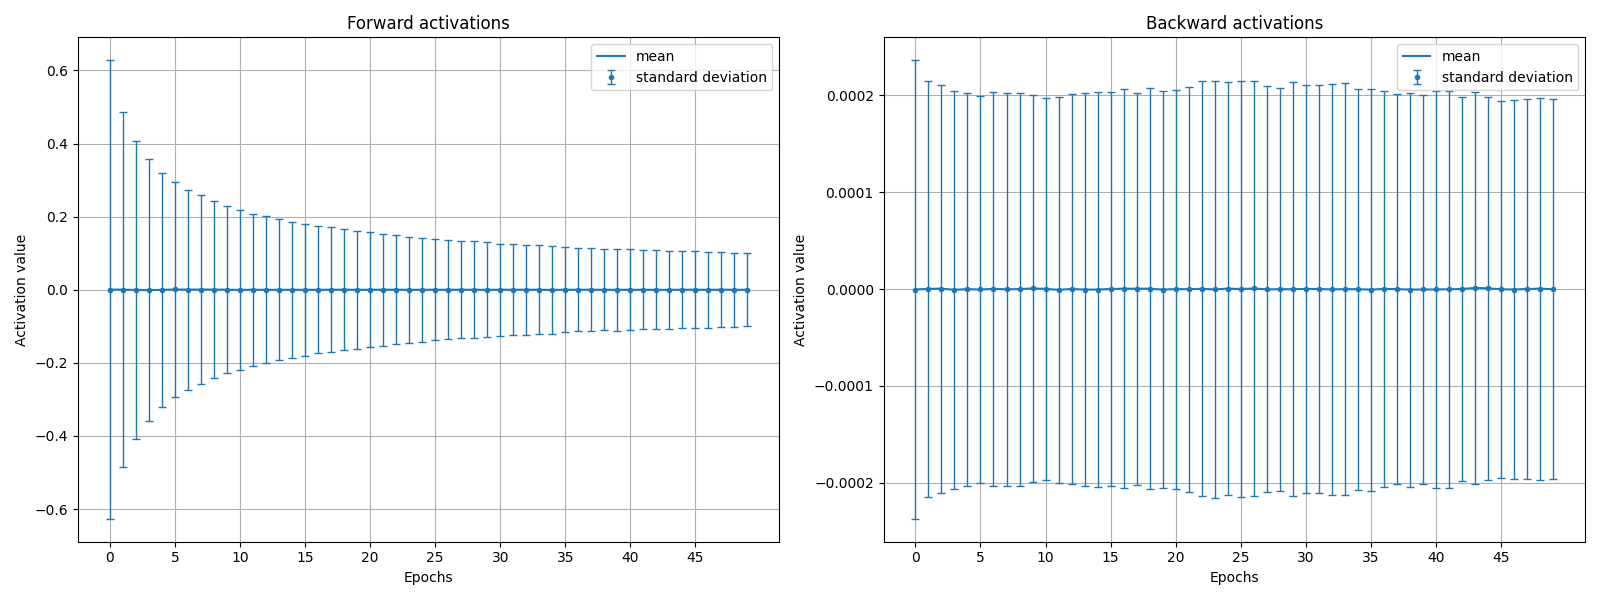
\includegraphics[width=\textwidth]{../out/01_deep/tanh_xavier_uniform.png}
        \caption{\textbf{Xavier uniform}}
    \end{subfigure}
    \begin{subfigure}[b]{0.95\textwidth}
        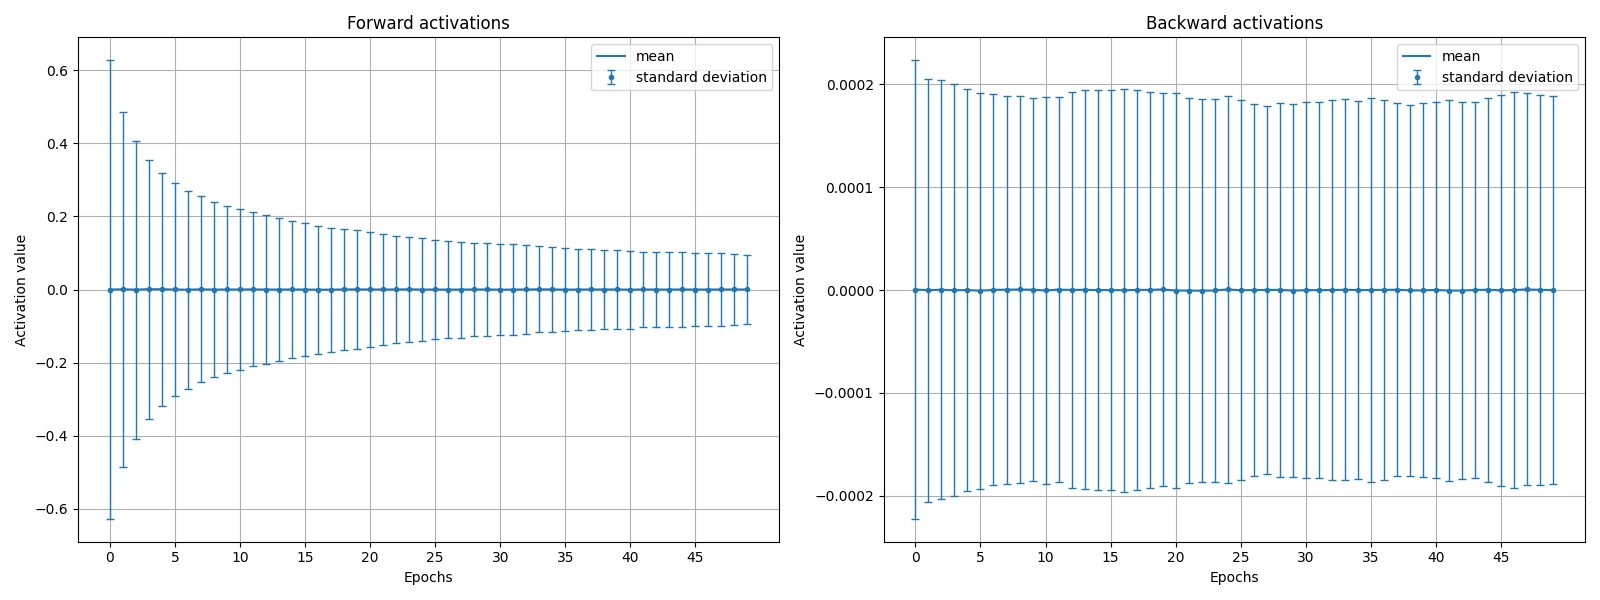
\includegraphics[width=\textwidth]{../out/01_deep/tanh_xavier_normal.png}
        \caption{\textbf{Xavier normal}}
    \end{subfigure}
    \caption{\textbf{Xavier} initialization used with \textit{tanh} activation}
    \label{fig:xavier_tanh}
\end{figure}

This initialization method looks much better than the original heuristic which is shown in figure \ref{fig:xavier_tanh}.
Even though the variance of the activations is decreasing, it is decreasing much more slowly and even in the last layer the variance is still significant.
The same can be said about gradients, whose variance almost does not change and its scale is reasonable, I would say.

From the graphs we can see only slight differences between the uniform and normal versions.
There is a slightly bigger variance of the gradients in the uniform case but the difference is tiny.
This method works really well for the \textit{tanh} activation function.

Now, we can try this method also for \textit{ReLU} activation.
This activation is very different from \textit{tanh} because it is not symmetric and half of the values are mapped to 0 and the other half is not bounded by 1.
This might cause problems for the \textbf{Xavier} initialization.

\begin{figure}[ht]
    \centering
    \begin{subfigure}[b]{0.95\textwidth}
        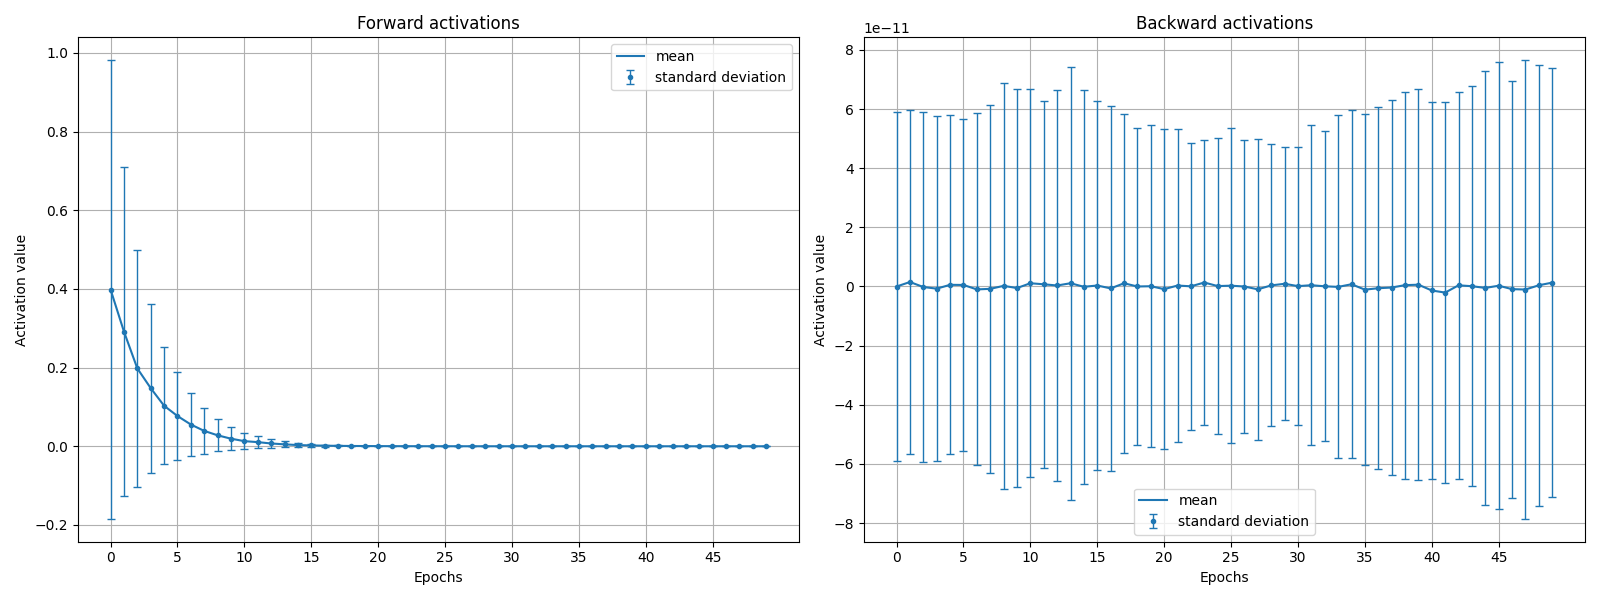
\includegraphics[width=\textwidth]{../out/01_deep/relu_xavier_uniform.png}
        \caption{\textbf{Xavier uniform}}
    \end{subfigure}
    \begin{subfigure}[b]{0.95\textwidth}
        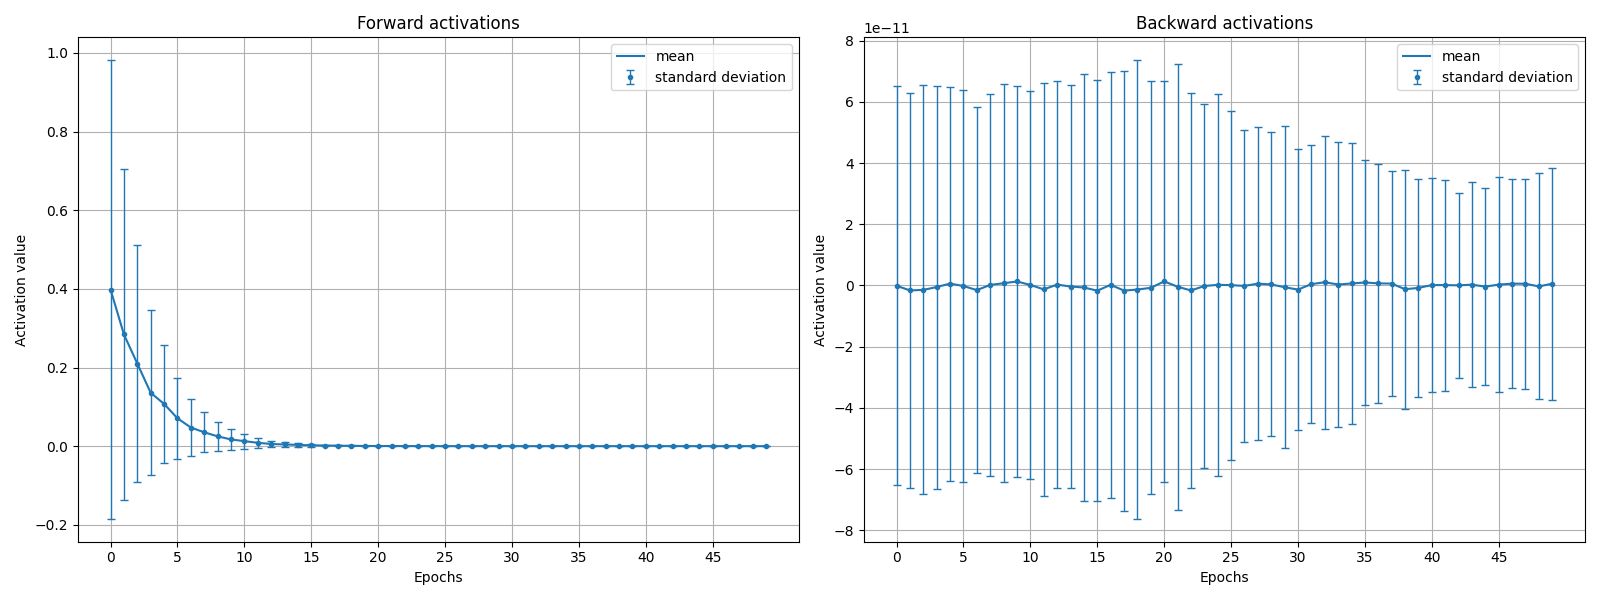
\includegraphics[width=\textwidth]{../out/01_deep/relu_xavier_normal.png}
        \caption{\textbf{Xavier normal}}
    \end{subfigure}
    \caption{\textbf{Xavier} initialization used with \textit{ReLU} activation}
    \label{fig:xavier_relu}
\end{figure}

From the graphs in figure \ref{fig:xavier_relu} we can confirm the ideas explained above.
The fact that half of the values is mapped to 0 and the other half is not bounded causes that the mean in the initial few layers is not zero, even thought the input vectors have zero mean.
The values can be only positive or zero, thus the mean must be also positive or zero.
In later layers this effect disappears and the mean goes to zero as well as the variance.
The statistics of the gradients have a similar problem to the original heuristic with \textit{tanh} activation and that is the scale.
The variance is of the order $10^{-11}$ which is again very slow and will probably not result in meaningful learning.
In the \textbf{Xavier normal} case it even looks like a gradient explosion because the variance is increasing but the scale is so small that we probably do not need to worry about it.

\subsection{Kaiming initialization}
In the previous case we verified a good method for initializing weights for the \textit{tanh} activation function.
However, that same method provided only poor results for the \textit{ReLU} activation, which is more popular in practice because it does not suffer from vanishing gradients.
There exists a method designed for this non-symmetric activation function with unbounded positive range of values which is called \textbf{Kaiming}.
Again, it has two versions, one for uniform and one for normal distribution.
So we again sample from the two most commonly used distributions but with different parameters.

\begin{figure}[ht]
    \centering
    \begin{subfigure}[b]{0.95\textwidth}
        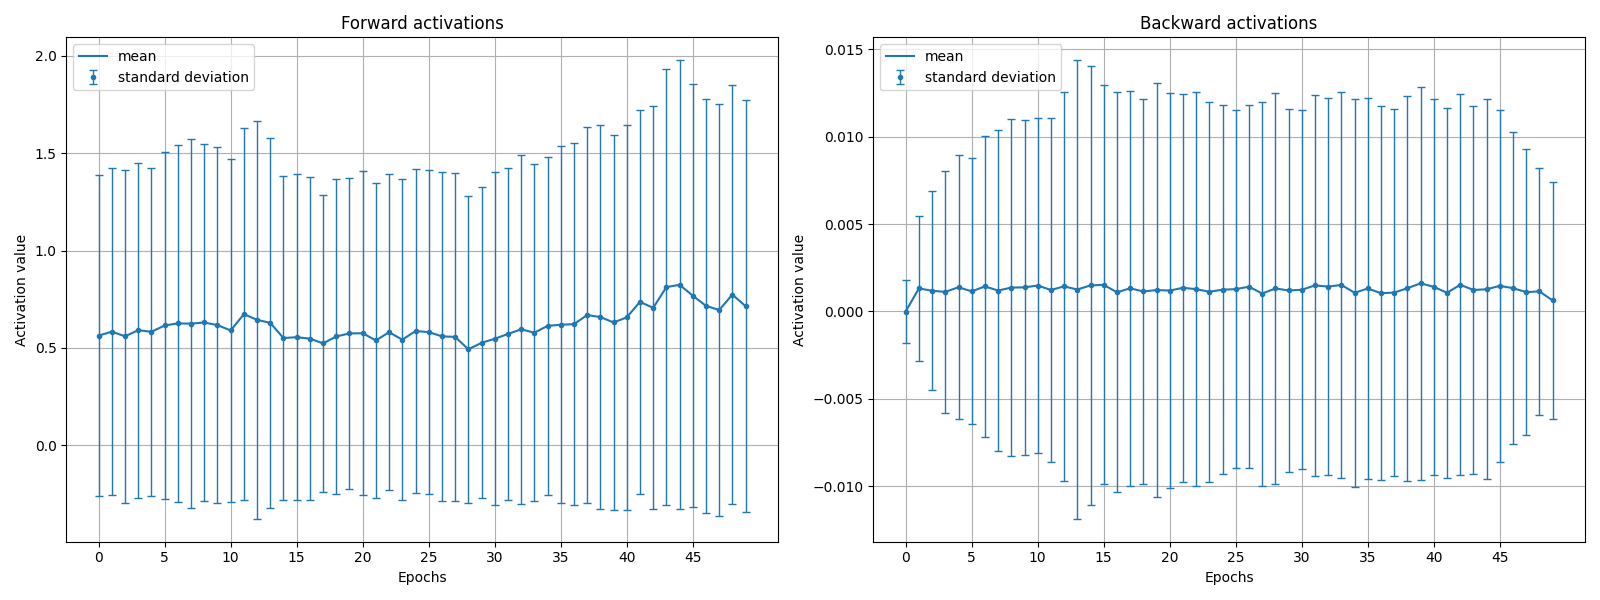
\includegraphics[width=\textwidth]{../out/01_deep/relu_kaiming_uniform.png}
        \caption{\textbf{Kaiming uniform}}
    \end{subfigure}
    \begin{subfigure}[b]{0.95\textwidth}
        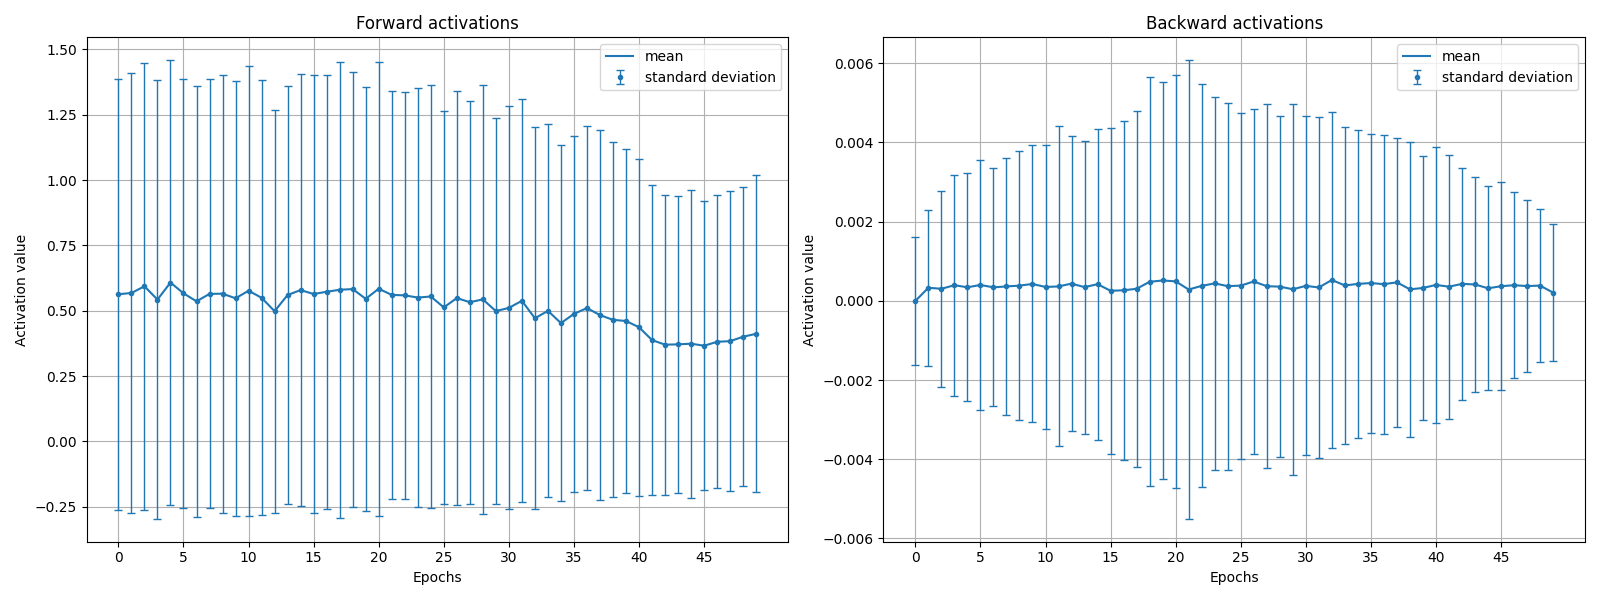
\includegraphics[width=\textwidth]{../out/01_deep/relu_kaiming_normal.png}
        \caption{\textbf{Kaiming normal}}
    \end{subfigure}
    \caption{\textbf{Kaiming} initialization used with \textit{ReLU} activation}
    \label{fig:kaiming_relu}
\end{figure}

The results in figure \ref{fig:kaiming_relu} show that this method works really well for the \textit{ReLU} activation function.
Even though the mean is not nicely close to zero as in the case of \textbf{Xavier} initialization for \textit{tanh} activation but it oscilates around $0.5$, the variance is kept smiliar to the variance of the input.
The reduction in magnitude of the variance is smaller than in the \textbf{Xavier} case but it looks less stable.

The gradients are very interesting.
The mean is above zero but only slightly which is nice.
However, the variance initially gets bigger in the few last layers, then stays roughly constant and then reduces as it approaches the input layer.
The \textbf{normal} case does not even have the constant part, it just increases towards roughly the middle layer and then decreases again.
I am not sure how to interpret it, it seems like the inner layers are learning faster than the input and output layers.

\subsection{Conclusion}
We have compared the three initialization methods for two commonly used activation functions and assessed their performance in terms of preserving the mean and variance of the input data throughout the network.
We can safely say that the choice of the initialization method is crucial for efficient learning of deep networks and that the method should be selected based on the activation function used.
The \textit{tanh} activation works great with both \textbf{Xavier} variants and the \textit{ReLU} activation works best with the \textbf{Kaiming} initialization.
\textit{ReLU} with \textbf{Xavier} methods fails because of the asymmetricity and diferent range of values.

\section{Initialization - Shallow Network}
In previous section, we studied the effects of different initialization methods on a deep network.
In this section, we aim to show negative effects such as exploding and vanishing gradients even if the initialization is done correclty.
More precisely, we will focus on statistics of the data itself and its normalization.

\subsection{Setup}
For this purpose we created a shallow network consisting of two linear layers followed by \textit{ReLU} activations.
The network acts on points $x \in \mathbb{R}^2$ generated by \texttt{CircleDataGenerator} provided in the template.
The first hidden layer has $6$ neurons, the second one has $3$ neurons and the output of the layer is $y \in \mathbb{R}^2$ becuase the dataset generates two classes.
We will turn this outputs into probabilities by \textit{softmax}.

Because we use the \textit{ReLU} activation function, we will use the \textbf{Kaiming} initialization method and we decided to use the \textbf{normal} variant.
The bias is initialized from the uniform distribution $U\left[-\frac{1}{\sqrt{n}}, -\frac{1}{\sqrt{n}}\right]$ where $n$ is the number of neurons in the previous layer.

It was suggested to use training set of size $100$ and to sample a sufficiently large validation set.
We used $50$ points for validation as in practice the validation set is usually smaller than the training set but it should also represent the data well.
In this case, we could have used more data as the dataset is small and not computationally heavy but we chose to stick with a more realistic setting.

For training, we used the suggested approach, that is to use the \textbf{AdamW} optimizer with learning rate $3e^{-4}$ using the whole data as one batch, using \textit{cross-entropy} loss and choosing quite big number of epochs.
It was suggested to use $5000$ epochs, in the end we used $10000$ epochs because the learning was still fast and we might see more things in longer learning.

There were three experiments with the same setup, they differed only in manipulating the input data before learning.
We show the results of these experiments below and the results are shown

\subsection{Experiments}

\begin{figure}[ht]
    \centering
    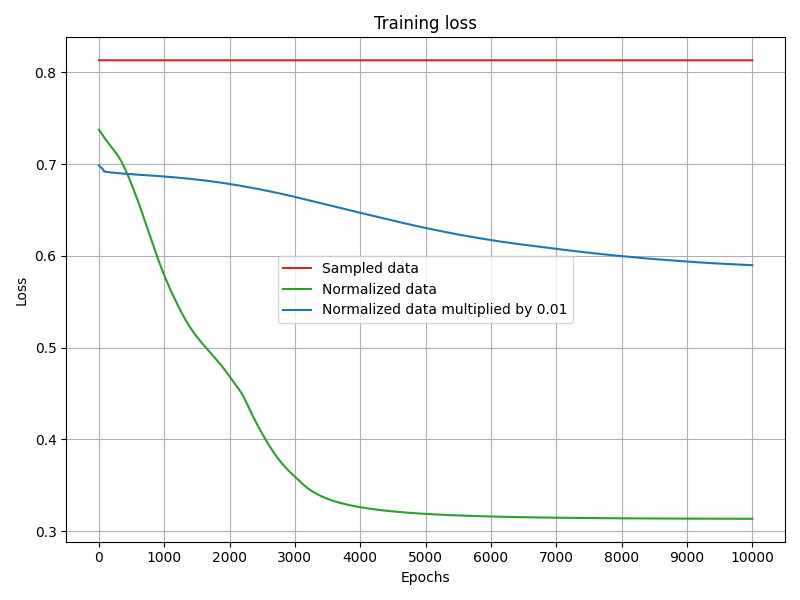
\includegraphics[width=0.5\textwidth]{../out/02_shallow/training_loss.png}
    \caption{Training loss of the three experiments}
    \label{fig:training_loss}
\end{figure}

The first experiment was to train the network on the sampled data without any manipulations and see what performance we can achieve.
The reults will be shown and summarized later but we want to add a quick note.
Sometimes it happened that the network did not learn at all because the weights were changing only very little and the loss was decreasing only by tiniest amounts.
In other rounds of training, it was learning something but still very slowly.
In the graph we have captured the case where there was almost no learning.
It seemed that it depends on the initialization of weights even though the method was the same for all experiments.
Thus the only explanation we have is that it depends on the random device and how the weights are sampled.

Second experiment was to first normalize the data to have zero mean and unit variance and the third task was to scale down the normalized data and see what the model learns.

Figure \ref{fig:training_loss} shows the training loss of the model during the three experiments.
As mentioned above, the first experiment with sampled data learns almost nothing, the changes cannot even be seen on the graph.
Normalizing the data, on the other hand, makes the network learn very well with the loss decreasing rapidly and smoothly.
Later we will show that the accuracy of the network corresponds to this result.

When we investigate the initial losses, as suggested by Karpathy, we can see why the data normalization matters.
In table \ref{tab:initial_losses} we can see that the initial loss for the original data is much higher than the expected loss.
Normalization of the data brings it closer and the scaling almost reaches it.
However, the scaling introduces other issues such as slow learning as can be seen from \ref{fig:training_loss} and the following graphs.

\begin{table}[ht]
    \center
    \begin{tabular}{| r | l |}
        \hline
        \textbf{Data}          & \textbf{Initial loss}                                       \\
        \hline
        \hline
        \textbf{Expected loss} & $-\log\left(\frac{1}{n_{\mathrm{classes}}}\right) = 0.6931$ \\
        \hline
        \hline
        Original data          & 0.8133                                                      \\
        Normalized data        & 0.7376                                                      \\
        Scaled normalized data & 0.6987                                                      \\
        \hline
    \end{tabular}
    \caption{Initial loss for differently manipulated data}
    \label{tab:initial_losses}
\end{table}

In figure \ref{fig:accuracy} we show the training and validation accuracies of the differently trained models.

\begin{figure}[ht]
    \centering
    \hfill
    \begin{subfigure}[b]{0.4\textwidth}
        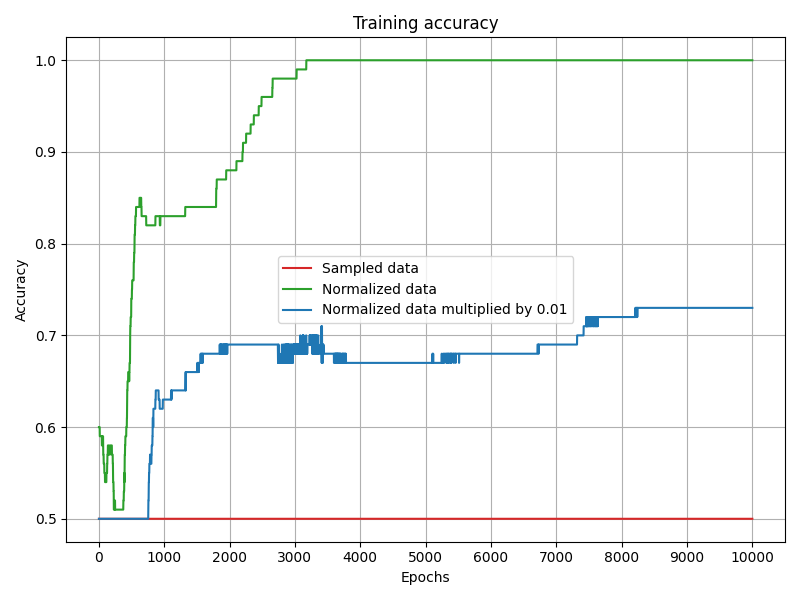
\includegraphics[width=\textwidth]{../out/02_shallow/training_acc.png}
        \caption{Training accuracy}
    \end{subfigure}
    \hfill
    \begin{subfigure}[b]{0.4\textwidth}
        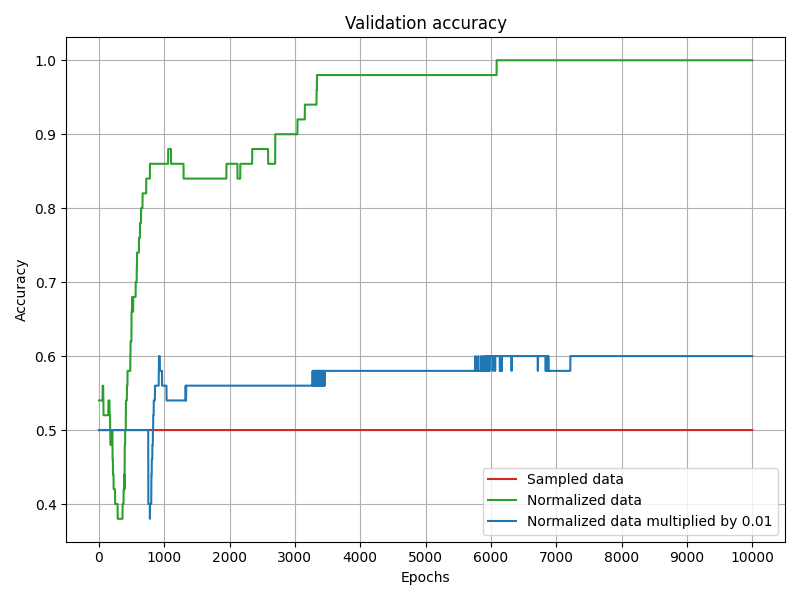
\includegraphics[width=\textwidth]{../out/02_shallow/validation_acc.png}
        \caption{Validation accuracy}
    \end{subfigure}
    \hfill
    \caption{Accuracies of the differently trained models}
    \label{fig:accuracy}
\end{figure}

It corresponds to the loss graphs in terms of the normalized model reaching full accuracy on both the training and validation sets, the scaled model increasing its accuracy but not fast enough and the original data model not improving at all becuase it is not learning much.
I reckon that if the training was longer, the scaled model could also reach high accuracy but it would take much longer because of the scaled data.
We can also show the decision boundaries for the different models and see what they learned, see figure \ref{fig:boundaries}.

\begin{figure}[ht]
    \centering
    \hfill
    \begin{subfigure}[b]{0.3\textwidth}
        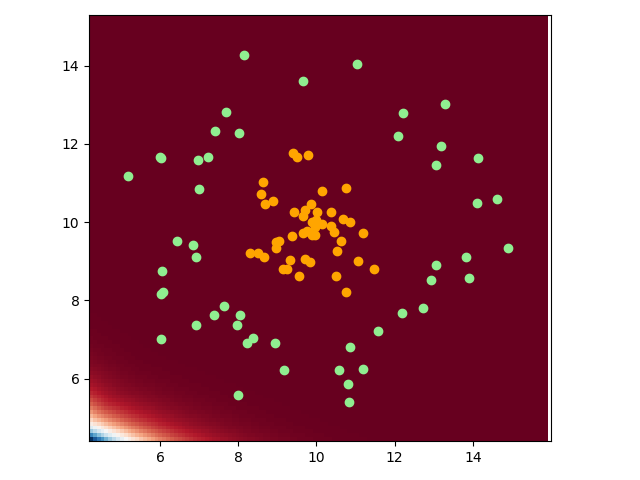
\includegraphics[width=\textwidth]{../out/02_shallow/original.png}
        \caption{Original data}
    \end{subfigure}
    \hfill
    \begin{subfigure}[b]{0.3\textwidth}
        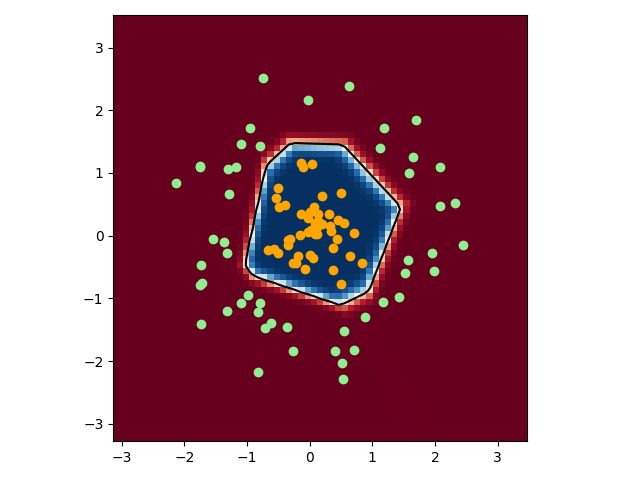
\includegraphics[width=\textwidth]{../out/02_shallow/norm.png}
        \caption{Normalized data}
    \end{subfigure}
    \hfill
    \begin{subfigure}[b]{0.3\textwidth}
        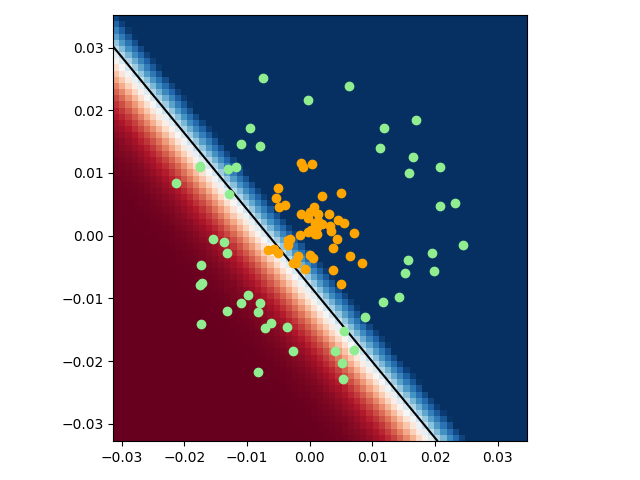
\includegraphics[width=\textwidth]{../out/02_shallow/mult.png}
        \caption{Scaled normalized data}
    \end{subfigure}
    \hfill
    \caption{Decision boundaries for the differently trained models}
    \label{fig:boundaries}
\end{figure}

The results in figure \ref{fig:boundaries} are as expected.
The normalized model learned to perfectly separate the two classes, the scaled model learns in a correct direction and the original model learns almost nothing.
To investigate possible reasons for this, we measured the norms of the gradients in the layers of the network and comapred them.
They can be seen in figure \ref{fig:grad_norms}.

\begin{figure}[ht]
    \centering
    \hfill
    \begin{subfigure}[b]{0.3\textwidth}
        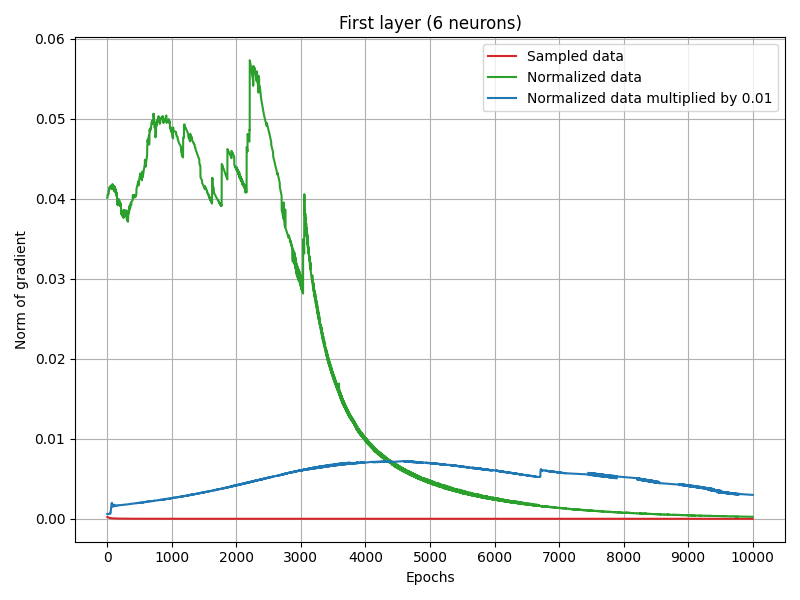
\includegraphics[width=\textwidth]{../out/02_shallow/grad_1.png}
        \caption{First layer (6 neurons)}
    \end{subfigure}
    \hfill
    \begin{subfigure}[b]{0.3\textwidth}
        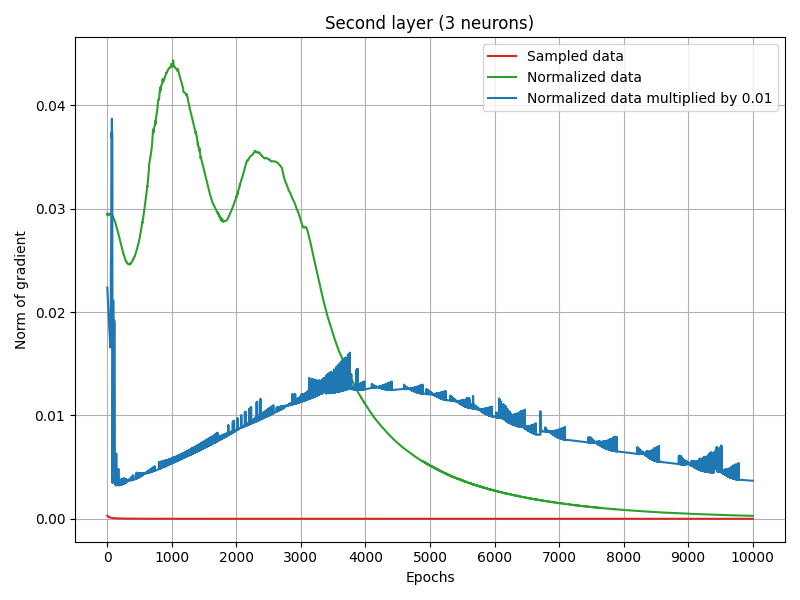
\includegraphics[width=\textwidth]{../out/02_shallow/grad_2.png}
        \caption{Second layer (3 neurons)}
    \end{subfigure}
    \hfill
    \begin{subfigure}[b]{0.3\textwidth}
        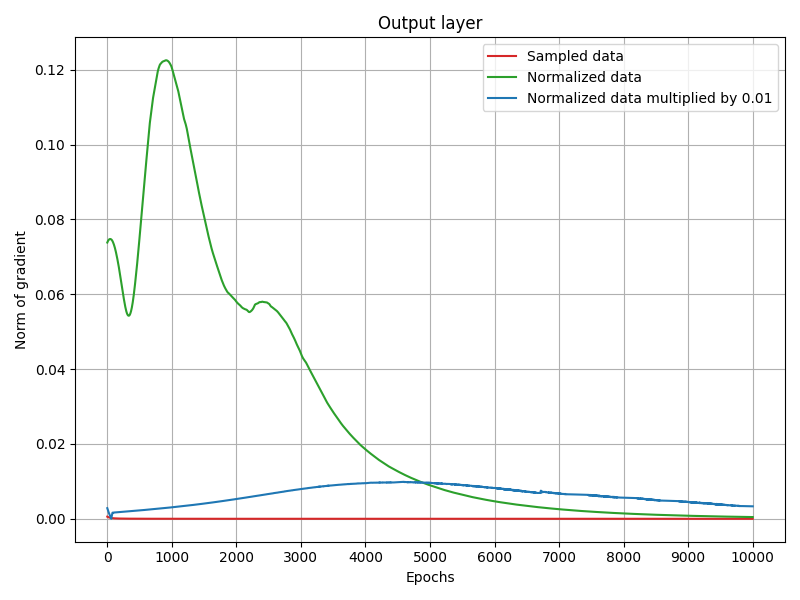
\includegraphics[width=\textwidth]{../out/02_shallow/grad_out.png}
        \caption{Output layer}
    \end{subfigure}
    \hfill
    \caption{Norms of gradients for individual layers in each epoch}
    \label{fig:grad_norms}
\end{figure}

These results show us where is the problem.
For all except the normalized case, the norm of the gradient is small during the whole training.
Combine it with a learning rate $< 1$ and the updates are even smaller.
Especially for the original data we can see that the gradients are almost zero which is the reason why the model is not learning.
Thus, we encountered vanishing gradients which can cause slow learning even in a case where the initial loss is almost exactly the same as the expected initial loss.
The weights are not updated fast enough.
If we carried out many more epochs, the scaled model probably could reach higher accuracy but it is not ideal.

\subsection{Conclusion}
In this section we have shown that a correct initialization is not always enough.
It also sometimes depends on the data itself.
We have shown that normalizing the data can vastly improve speed of learning and reaching high accuracy.
We must be careful about the scales of the data and weights so that the gradients are not too small and do not vanish.

\section{Regularization - Dropout}
In the last task, we explore the effects of using dropout layers as a regularization technique in neural networks.
We will work with the famous \textbf{MNIST} dataset.
The loading and transformation was prepared in the template so we will just use that.

First, we prepare the network with input size $28 \times 28 = 784$ and output size $10$.
Note, that the input images are square matrices, so we must flatten them to a single feature vector.
In the assignment, there is not mentioned any activation so initially we tried training the networks without activations, which did not seem right.
The results were as expected, the network with dropout was significantly better than the one without dropout.
The results can be seen in figure \ref{fig:mnist_no_act}.

\begin{figure}[ht]
    \centering
    \hfill
    \begin{subfigure}[b]{0.45\textwidth}
        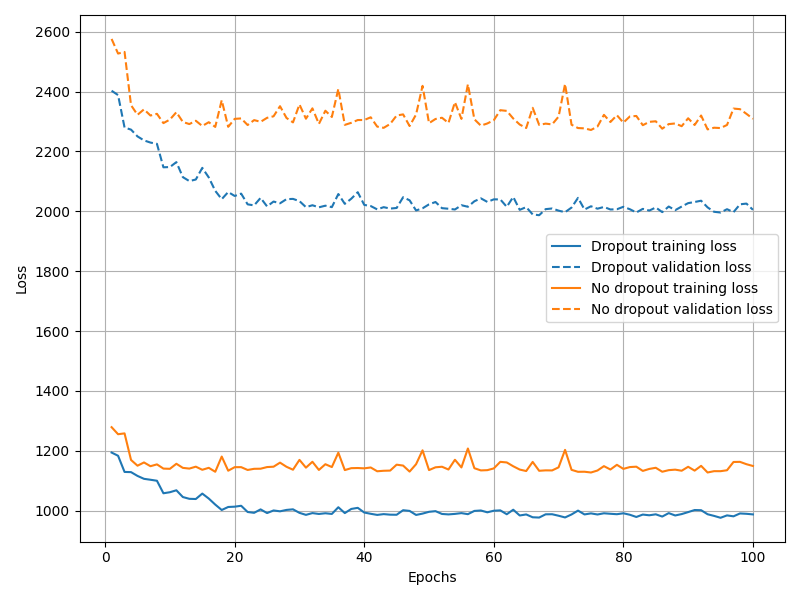
\includegraphics[width=\textwidth]{../out/03_dropout_no_relu/loss.png}
        \caption{Losses}
    \end{subfigure}
    \hfill
    \begin{subfigure}[b]{0.45\textwidth}
        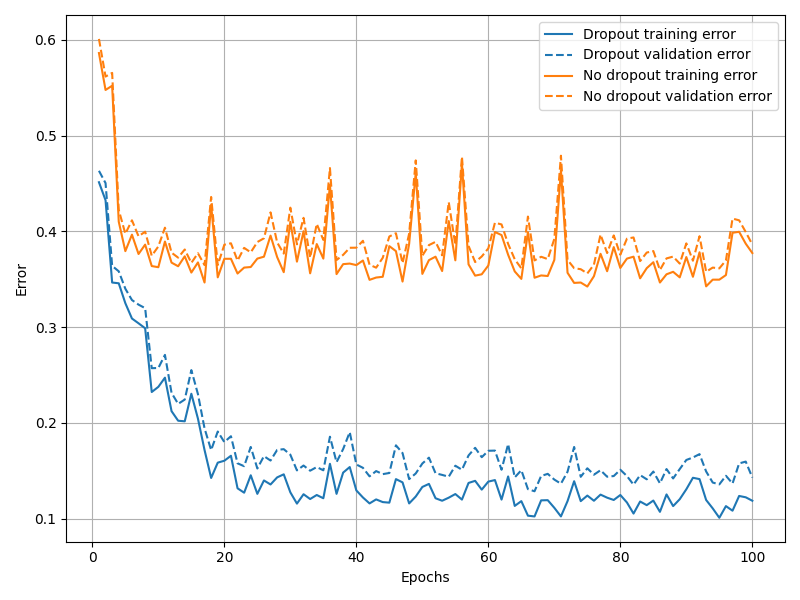
\includegraphics[width=\textwidth]{../out/03_dropout_no_relu/error.png}
        \caption{Errors}
    \end{subfigure}
    \hfill
    \caption{Training the network without activations}
    \label{fig:mnist_no_act}
\end{figure}

However, training without activation does not make sense to us so we added \textit{ReLU} activation after each dropout layer.
We chose \textit{ReLU} because the network is shallow enough so that the normal initialization should not be an issue and it is a commonly used activation.
The results were significantly better than without activation but they were not as we expected as can be seen in \ref{fig:mnist_activation}.
The network without dropout slightly outperformed the network with dropout both on the validation set and on the test set.
It also converged slightly faster.

\begin{figure}[ht]
    \centering
    \hfill
    \begin{subfigure}[b]{0.45\textwidth}
        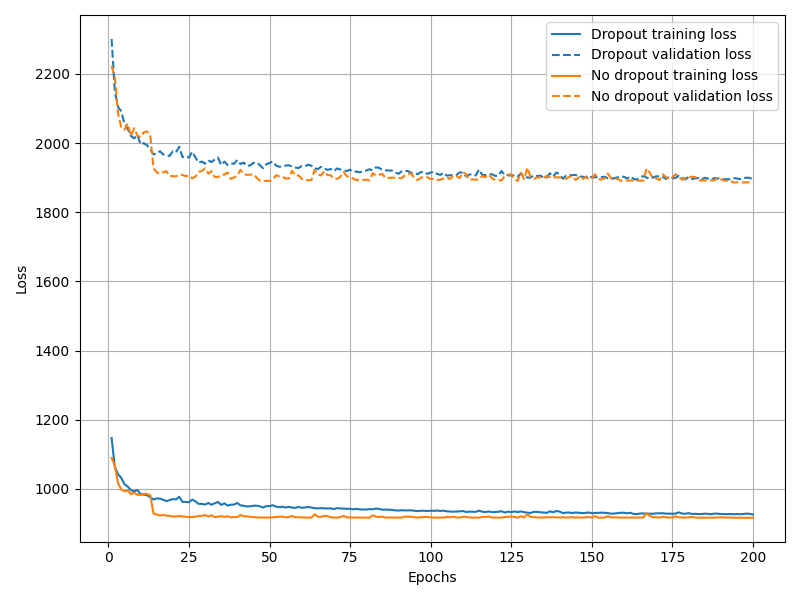
\includegraphics[width=\textwidth]{../out/03_dropout/loss.png}
        \caption{Losses}
    \end{subfigure}
    \hfill
    \begin{subfigure}[b]{0.45\textwidth}
        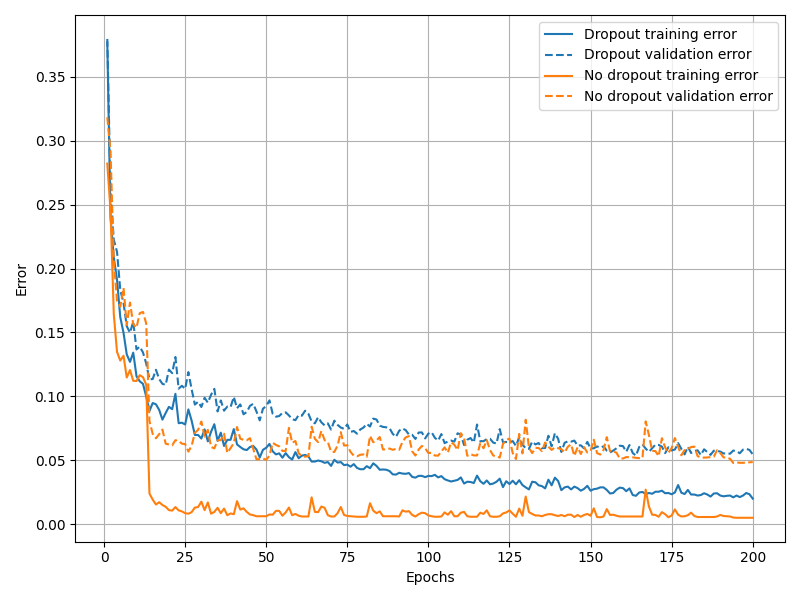
\includegraphics[width=\textwidth]{../out/03_dropout/error.png}
        \caption{Errors}
    \end{subfigure}
    \hfill
    \caption{Training the network with \textit{ReLU} activations}
    \label{fig:mnist_activation}
\end{figure}

I am not sure why is that, if we were not supposed to used activations, then the layer without dropout is technically just one linear layer so it cannot be so.
The purpose of dropout is, to my understanding, to prevent overfitting and make the network generalise better.
In this case, both networks generalize well on the test set so maybe it does not make a big difference.

Lastly, we were supposed to construct ensamble models of the dropout model and report the classification errors.
We put them together with the test errors of the other models into table \ref{tab:errors}.

\begin{table}
    \centering
    \begin{tabular}{| l | c | c |}
        \hline
        \textbf{model}    & \textbf{test error} & \textbf{test loss} \\
        \hline
        \hline
        dropout $p=0.5$   & $0.0514$            & $1890.4236$        \\
        \hline
        no dropout $p=0$  & $0.0468$            & $1883.7531$        \\
        \hline
        \hline
        ensamble $n=10$   & 0.0569              &                    \\
        ensamble $n=50$   & 0.0548              &                    \\
        ensamble $n=100$  & 0.0533              &                    \\
        ensamble $n=500$  & 0.0534              &                    \\
        ensamble $n=1000$ & 0.0536              &                    \\
        ensamble $n=2000$ & 0.0535              &                    \\
        \hline
    \end{tabular}
    \caption{Test errors and losses for dropout models}
    \label{tab:errors}
\end{table}

\subsection{Conclusion}
In this section, we explored the effects of using dropout layers in a neural network on the \textbf{MNIST} dataset.
We trained the same network with dropout enabled with probability $p=0.5$ and with dropout disabled.
From the results, the dropout did not do much in our case and the network without dropout was even slightly better on the test set.
This is not what we expected.

From the graphs of training loss and errors in figure \ref{fig:mnist_activation}, it is possible to deduce that if the learning was to continue for more epochs, the regularized model would probably get better while the non-regularized model seems to stagnate already.

\end{document}
